\newpage
\section{First section}

\subsection{Evo-RoleMiner Algorithm}
\begin{algorithm}
   	\caption{Evolutionary algorithm for single objectives}
   	\label{alg:EA}
   	\begin{algorithmic}[1]
   		\Procedure{eaSingle}{$popSize$, $NGEN$, $CXPB$, $MUTPB$}
   		\State $P_p$ = generatePopulation($popSize$)
   		\State evaluateIndividuals($P_p$)
   		\State $solutionFound$ = False
   		\State $generation$ = 1
   		\While{not $solutionFound$ AND $generation <= NGEN$}
   		\State $P_p$ = select($population$, k=length($P_p$))
   		\State $P_o$ = clonePopulation($P_p$)
   		\State $i$ = 0
   		\While{ $i < length(P_o)-1$}
   		\State $P_o$[$i$],$P_o$[$i$+1] = crossover($P_o$[$i$],$P_o$[$i$+1],$CXPB$)
   		\State $i$ += 2
   		\EndWhile
   		\State $i$ = 0
   		\While{ $i < length(P_o)$}
   		\State $P_o$[$i$] = mutation($P_o$[$i$],$MUTPB$)
   		\State $i$ += 1
   		\EndWhile
   		\State $P_p$ = $P_o$
   		\State evaluateIndividuals($P_p$)
   		\State $generation$ += 1
   		\EndWhile
   		\State \Return $result$
   		\EndProcedure
   	\end{algorithmic}
\end{algorithm}
The algorithm starts with the initial generation and evaluation of the parent population $P_p$. Then, for each generation, individuals from $P_p$ are selected and cloned as offspring population $P_o$. A loop over neighboring individuals in $P_o$ is mating individuals $\mathbf{x}_i$ and $\mathbf{x}_{i+1}$ by crossover probability $CXPB$. The resulting children $\mathbf{y}_i$ and $\mathbf{y}_{i+1}$ replace their respective parents in $P_o$. In a second loop over all individuals in $P_o$ the individuals get mutated by mutation probability $MUTPB$. The resulting mutation is replacing the original individual. The resulting individuals in $P_o$ can be generated from crossover only, mutation only, crossover and mutation, and reproduction according to the given probabilities $CXPB$ and $MUTPB$. The offspring population $P_o$ is then getting the parent population $P_p$ for the next generation, after each individual got evaluated.

\subsection{Data Generator}
\label{sec:dataGenerator}
Some papers are providing data generators for synthetic datasets for the performance evaluation of the various role mining algorithms. The data generator in Vaidya et al.\cite{Vaidya:2006:RMR:1180405.1180424} takes as input the number of users, permissions and roles to generate a pair of User-Role-Assignment and Role-Permission-Assignment matrices. Combining these two matrices, the corresponding User-Permission-Assignment matrix is obtained.\\
These data generators only consider users, permissions and their assignment to each other. They do not consider user attribute information. Due to this a new synthetic data generator has been created for this thesis, where the dimensions of users and permissions can be defined. The data generator is based on a reversed role-engineering process and generates users, roles, rules, user-role matrix, role-permission matrix, user-permission matrix and a user-permission matrix with noise.
\begin{itemize}
	\item \textbf{Generation of users}\\
	Given a user count $u$ and a list of user attributes $attr$ containing a list of user attribute values each, $u$ users are generated. A user is described by a list of user attributes, which have a specific user attribute value assigned. For example:\\
	\storestyleof{itemize}
	\begin{listliketab}
		\begin{tabular}{ll}
			Given   &  $attr$ = [$OrganizationalUnit$,$Location$,$EmployeeType$]\\
			where   &  $OrganizationalUnit$ = [$HumanResources$,$Sales$,$Motor$],\\
			&  $Location$ = [$Denmark$, $Germany$, $US$] and\\
			&  $EmployeeType$ = [$Internal$,$External$]\\
		\end{tabular}
	\end{listliketab}\\
	An user can be generated as follows: $user_1$ = [$Sales$,$Denmark$,$Internal$]. An additional parameter for a usertype count $t$ determines how many different users can exist. This ensures that users with the same user attributes can occur several times.
	
	\item \textbf{Generation of roles}\\
	Given a permission count $p$ and a role count $r$, $r$ roles are generated, which are described by a set of permissions from the range [1;$p$]. For example given $p$=7 a role can be: $role_1$ = \{$1$,$5$,$7$\}. A parameter $max_p$ limits how often a permission can occur in all $r$ roles. Additionally a configuration list $conf_p$ can regulate the density of roles. A configuration list entry contains 1) a percentage of all roles, which are affected by this configuration entry 2) the minimum count of permissions the role must have and 3) the maximum count of permissions the role must have. For example the configuration list [(0.2,10,20),(0.8,1,5)] would describe the configuration that 20\% of the $r$ roles must have between 10 and 20 permissions and the other 80\% of the $r$ roles must have between 1 and 5 permissions.
	
	\item \textbf{Generation of rules}\\
	\hl{UPDATE}
	Given a role count $r$ and a list of user attributes $attr$ containing a list of user attribute values each, $r$ rules are generated (a rule for each role). A rule is a list of user attributes, which have no, one or several user attribute values assigned. For example given the user attributes $attr$ from above, $rule_1$ = [\{$HumanResources$\}, \{$Denmark$,$Germany$\}, \{\}] would describe the rule $HumanResources \wedge (Denmark \vee Germany)$. A parameter for the maximal condition count $cond_{max}$ configures how many user attributes can be filled with values. The example $rule_1$ has currently two conditions: One for $OrganizationalUnit$ and one for $Location$.\\
	This rule is assigned to a role. Rules are generated until:
	\subitem \textbullet \space each role has a rule assigned
	\subitem \textbullet \space each generated user is meeting one rule
	\subitem \textbullet \space each rule is met by at least one user
\end{itemize}
Since users and roles have been generated before, the rules can be applied to create the following outputs:
\begin{itemize}
	\item \textbf{User-role matrix}\\
	The User-role matrix is a boolean matrix, where the rows are users and the columns are roles. A "1" in the matrix would mean that the user (row) is assigned to a the role (column). The users get those roles assigned, which have a rule assigned the user is fullfilling. For example $user_1$ would not fulfill $rule_1$, since the first condition for OrganizationalUnit is not met. The user $user_2$ = [$HumanResources$,$Denmark$,$Internal$] on the other hand would met the conditions in $rule_1$ and would therefore get get according role assigned.
	\item \textbf{Role-permission matrix}\\
	The Role-permission matrix is a boolean matrix, where the rows are roles and the columns are permissions. A "1" in the matrix would stand for that the role (row) is containing the permission (column). The matrix is generated from the generated roles.
	\item \textbf{User-permission matrix}\\
	The User-permission matrix is a boolean matrix, where the rows are users and the columns are permissions. A "1" in the matrix would imply that the user (row) is has the permission (column). The matrix is generated from the matrix multiplication of the User-role matrix and the Role-permission matrix.
	\item \textbf{User-permission matrix with noise}\\
	Given two parameters for noise, random bits in the User-permission matrix are flipped. The first parameter is the probability that a user-permission-relation is removed ("1" flipped to "0") and the second parameter is the probability that a user-permission-relation is added ("0" flipped to "1").
\end{itemize}

\subsection{Real Datasets}
\label{sec:visualRealDatasets}
\begin{figure}[H]
	\centering
	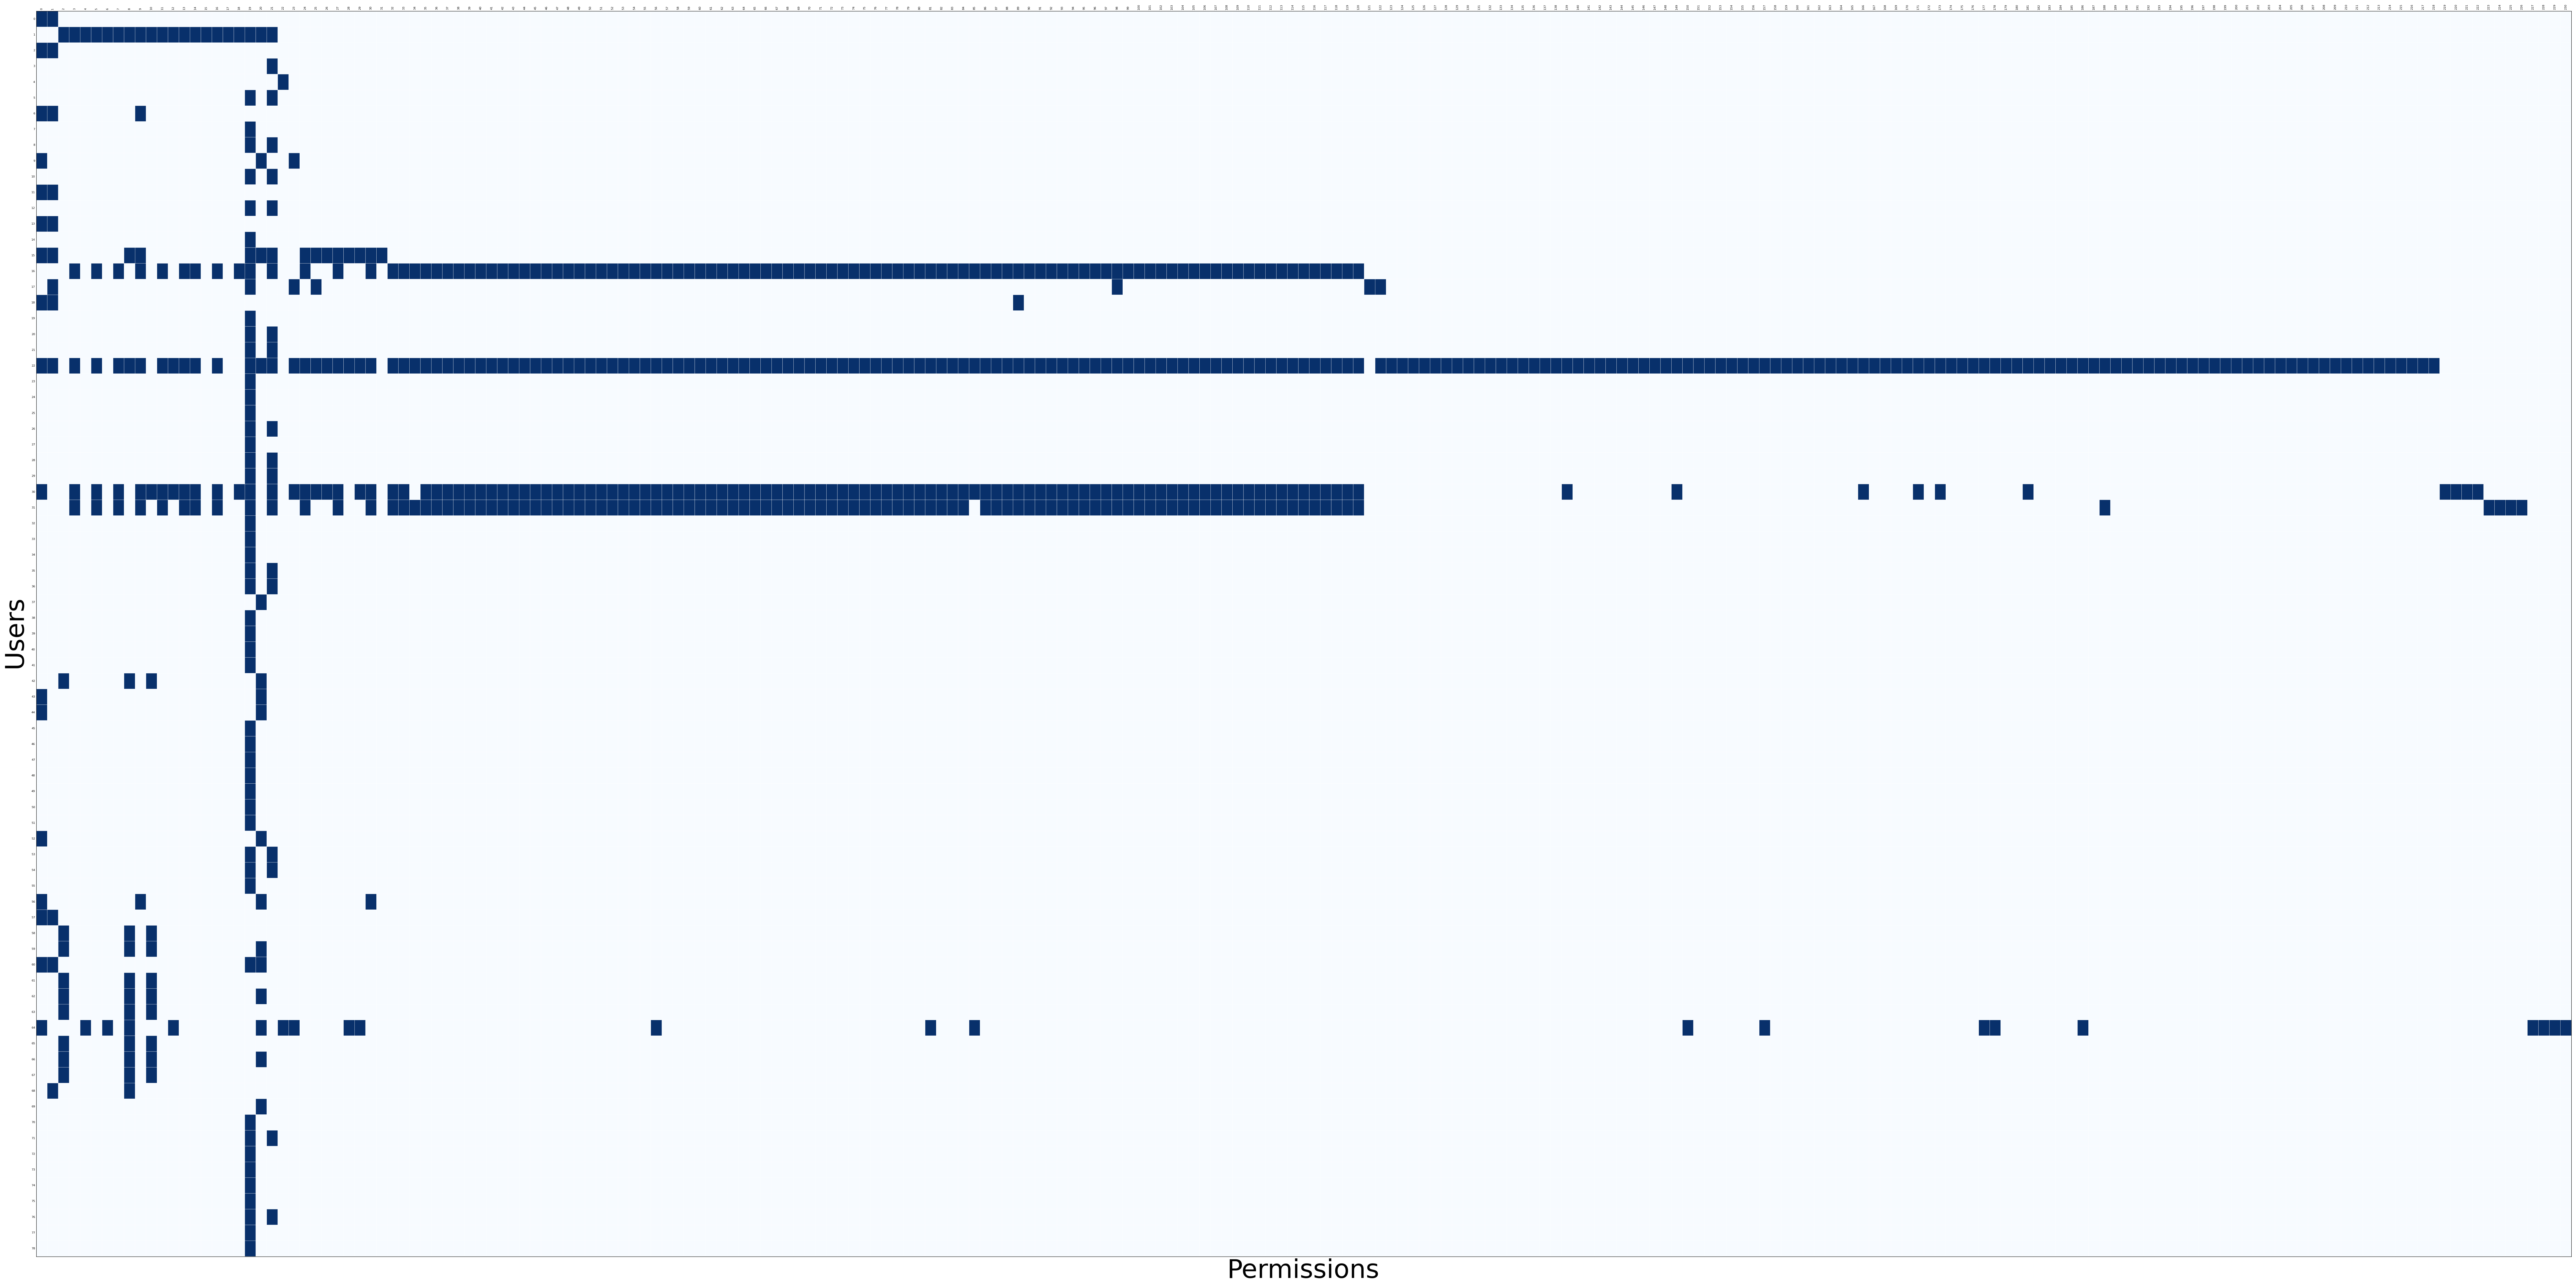
\includegraphics[scale=0.048]{./Figures/domino}
	\caption{DOMINO}
	\label{fig:domino}
\end{figure}
\begin{figure}[H]
	\centering
	
\includegraphics[scale=0.05]{./Figures/emea}
	\caption{EMEA}
	\label{fig:emea}
\end{figure}
\begin{figure}[H]
	\centering
	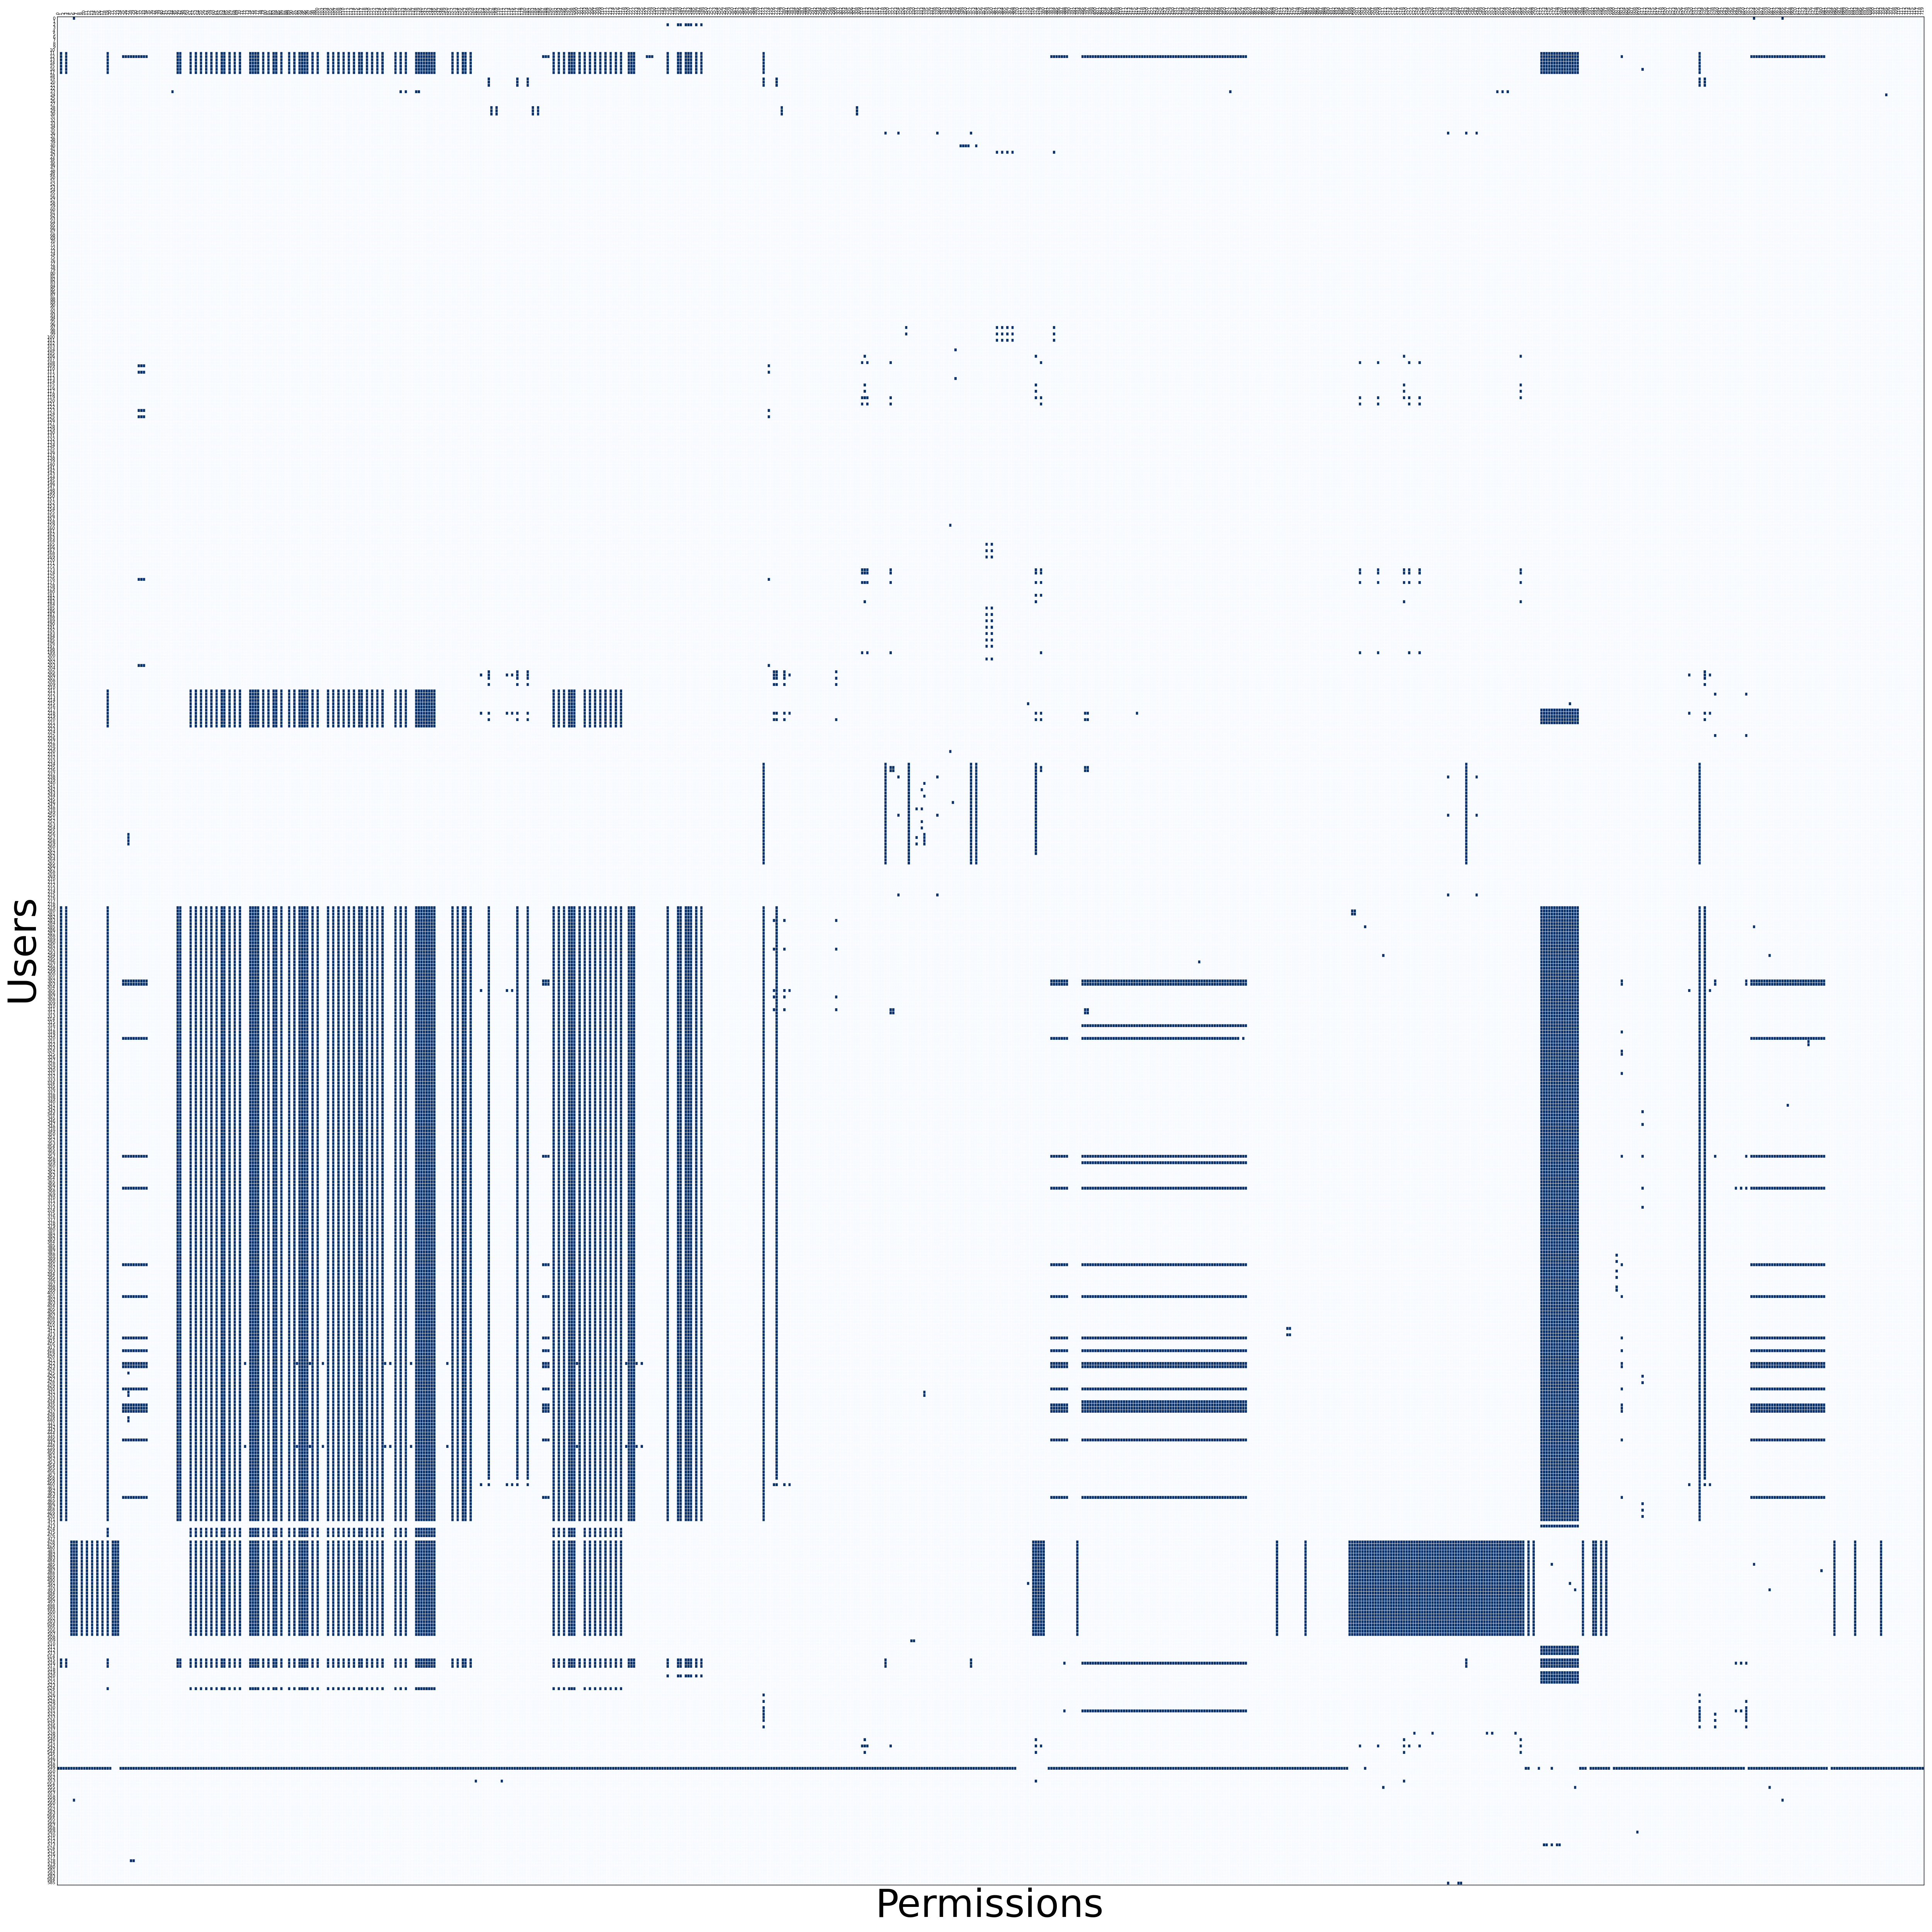
\includegraphics[scale=0.1]{./Figures/firewall1}
	\caption{FIREWALL1}
	\label{fig:firewall1}
\end{figure}
\begin{figure}[H]
	\centering
	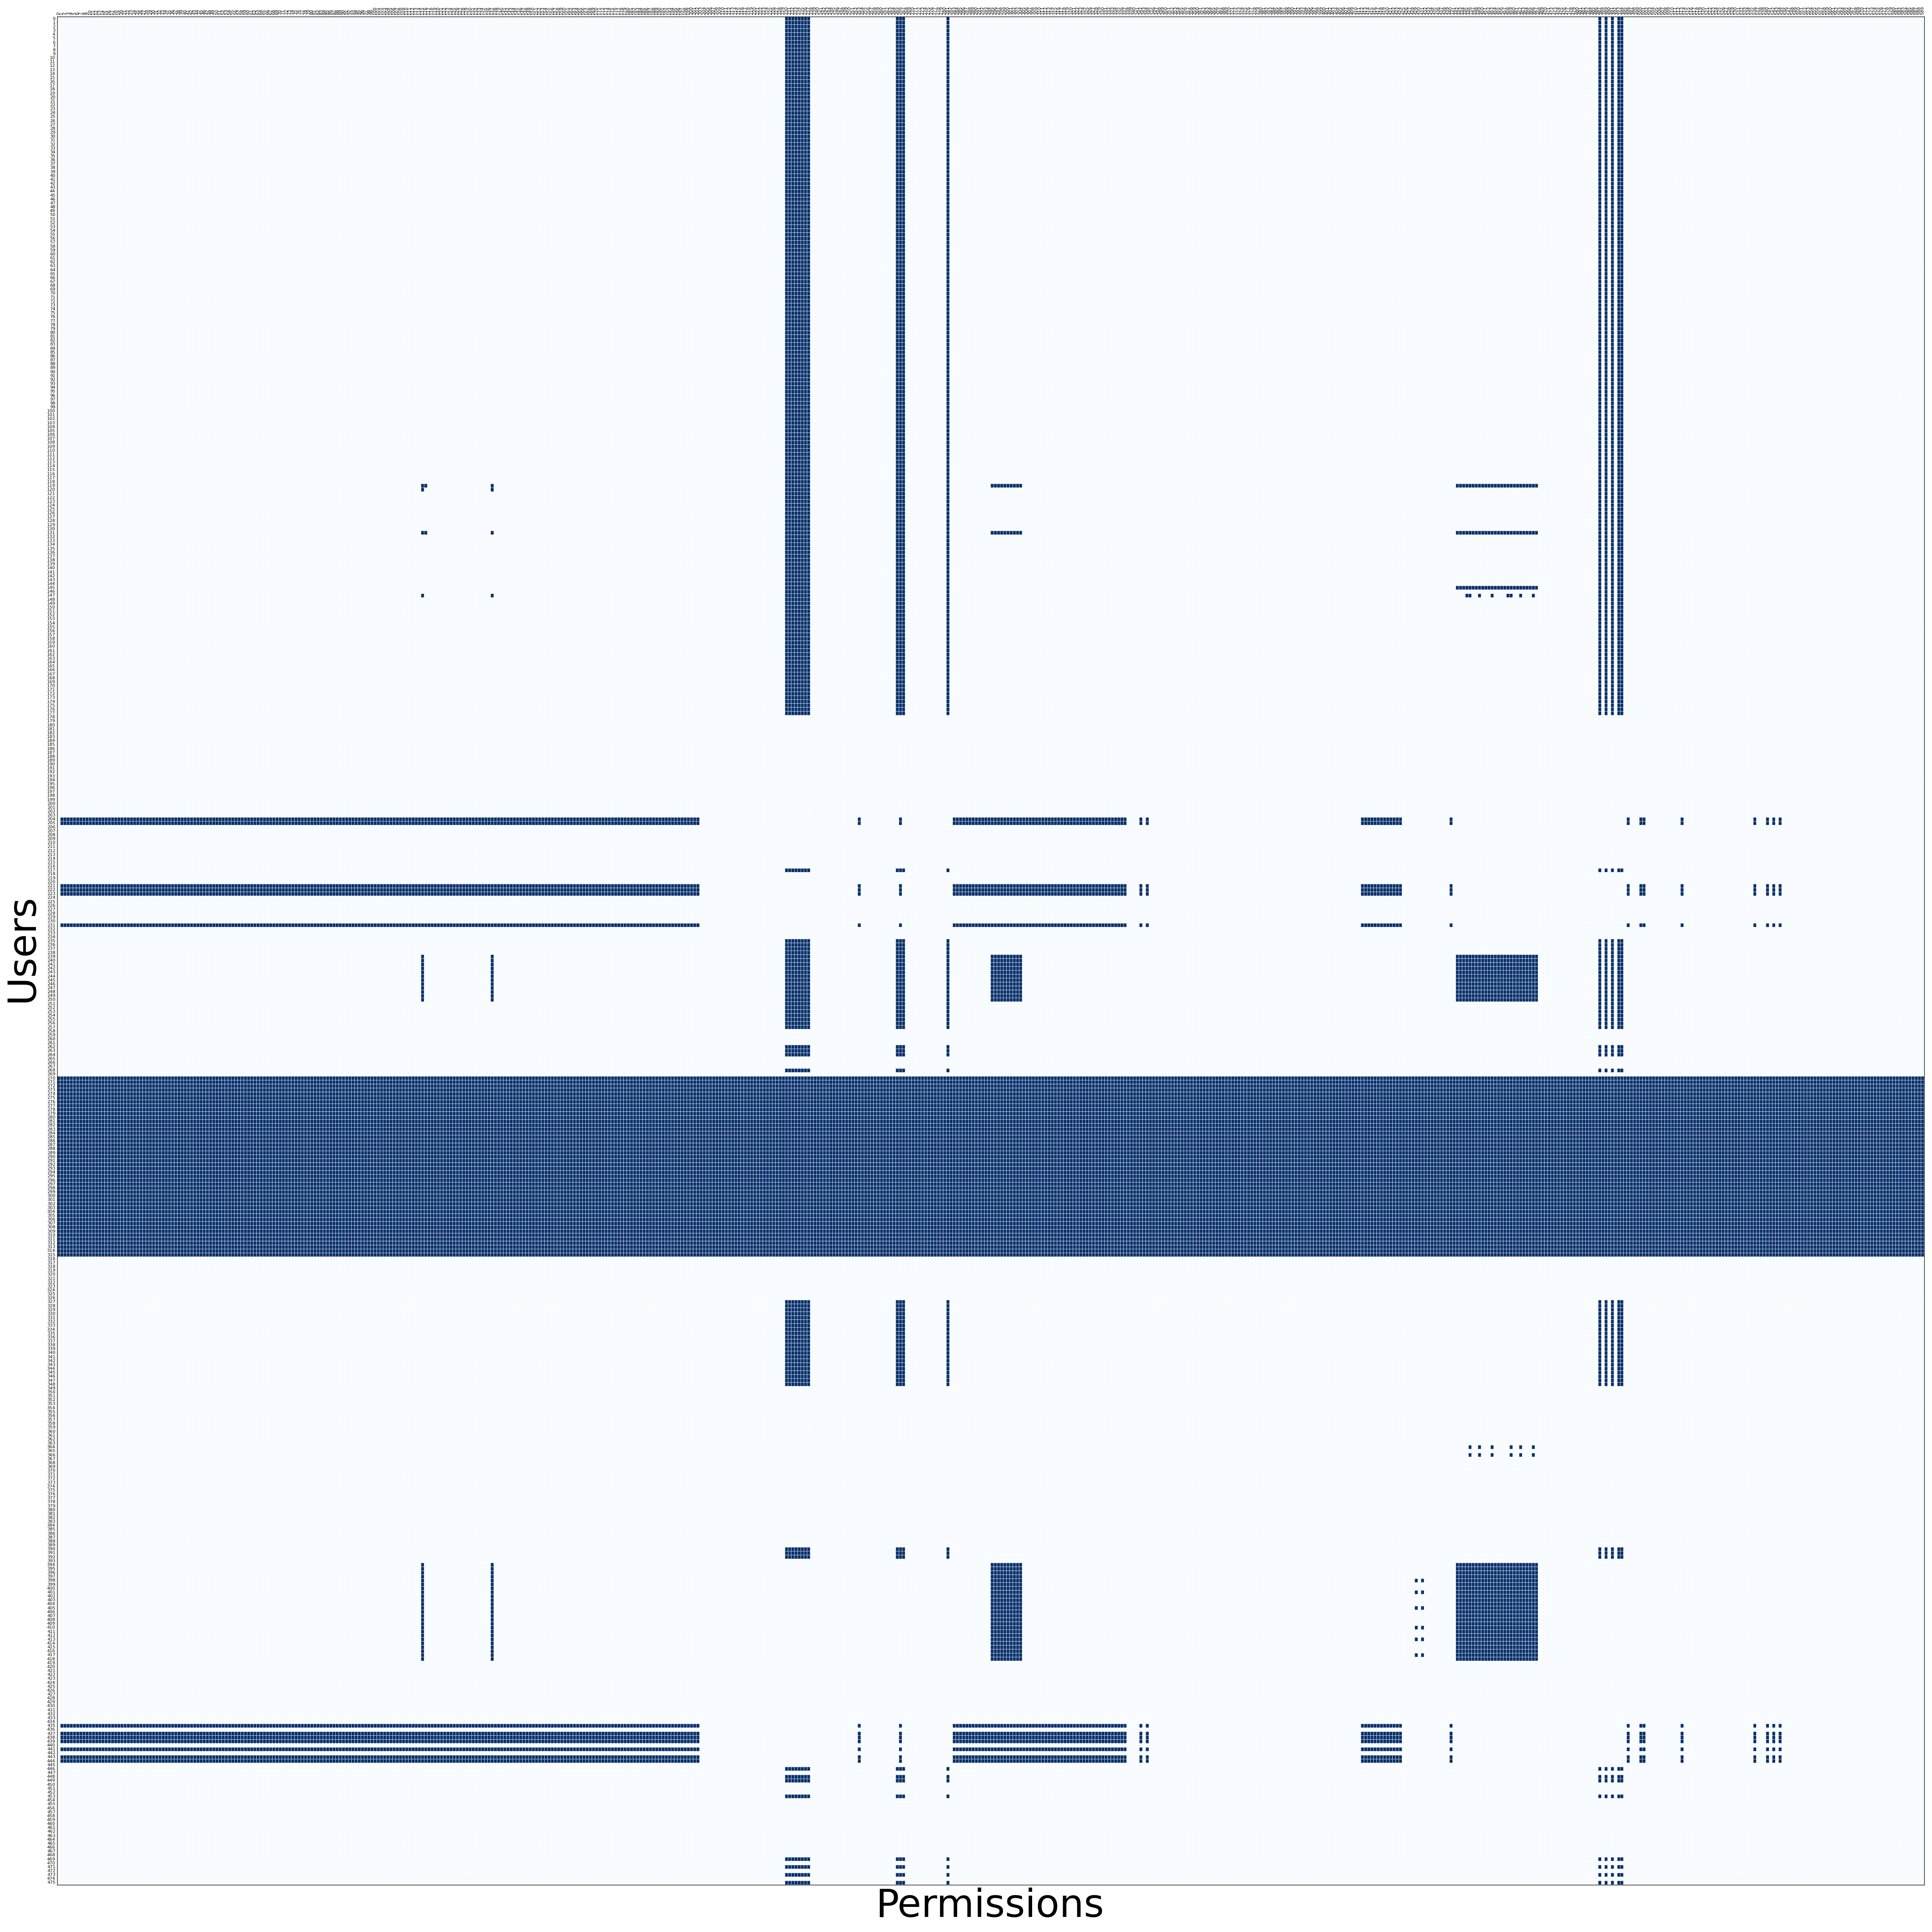
\includegraphics[scale=0.1]{./Figures/firewall2}
	\caption{FIREWALL2}
	\label{fig:firewall2}
\end{figure}

\subsection{Synthetic Datasets}
\label{sec:infoSyntheticDatasets}

\subsection{Implementation}
Implementation with the DEAP Framework for Python \cite{DeRainville:2012}